% !TEX option = --shell-escape
% !TEX program = xelatex
\documentclass[fontset=fandol]{ctexart}

\setmainfont{Linux Libertine O}
\setsansfont{Linux Biolinum O}

\usepackage{ragged2e}
\usepackage[svgnames]{xcolor}
\usepackage{pgfornament-han}
\usetikzlibrary{chains}
\usetikzlibrary{calc}
\usetikzlibrary{decorations}
\usetikzlibrary{decorations.text,decorations.markings}

\usepackage{cncolours}

\usepackage{geometry}
\geometry{hmargin=1in,vmargin=0.8in,headheight=10pt}
\usepackage{enumitem}
\usepackage{tcolorbox}
\tcbuselibrary{skins,raster}

%%%%%% 这段代码可以忽视,只是 --shell-escape 时调用 minted 不然就用 listings
\ifnum\shellescape=1
  \tcbuselibrary{minted}
  \setminted{breaksymbolleft={},breakindent=\ccwd}
  \newminted{latex}{}
  \newmintinline{latex}{}
\else
  \tcbuselibrary{listings}
  \newcommand{\latexinline}[1]{\lstinline|#1|}
  \lstnewenvironment{latexcode}{\lstset{language={[LaTeX]TeX}}}{}
  \lstset{basicstyle=\ttfamily}
\fi
%%%%%%%%


\tcbset{fonttitle=\kaishu\large\bfseries,colback=铅白!60!white,colbacktitle=绀青,coltitle=精白,colframe=墨灰}

\makeatletter
\newcommand{\getpgfornamenthanDim}[1]{%
 {\@pgfornamenthanDim{#1}宽:\@pgfornamentX\\高:\@pgfornamentY}%
}
\makeatother

\usepackage{fancyhdr}
\fancyhf{}
\renewcommand{\headrule}{}

\fancyhead[L]{%
\newbox{\fortyseven}
\savebox{\fortyseven}{\pgfornamenthan[scale=0.2,color=鸭卵青]{47}}
\tikzset{every node/.append style={inner sep=0pt,鸭卵青}}
\begin{tikzpicture}[overlay,remember picture]
\node[anchor=north west,shift={(14.5pt,-14.5pt)}] at (current page.north west)
  (nw) {\pgfornamenthan[scale=0.2]{25}};
\node[anchor=north east,shift={(-14.5pt,-14.5pt)}] at (current page.north east)
  (ne) {\pgfornamenthan[scale=0.2,symmetry=v]{25}};
\node[anchor=south west,shift={(14.5pt,14.5pt)}] at (current page.south west)
  (sw) {\pgfornamenthan[scale=0.2,symmetry=h]{25}};
\node[anchor=south east,shift={(-14.5pt,14.5pt)}] at (current page.south east)
  (se) {\pgfornamenthan[scale=0.2,symmetry=c]{25}};
%
\begin{scope}[start chain,node distance=0pt]
\node[anchor=north west,on chain] at (nw.north east) {\usebox{\fortyseven}};
\foreach \i in {1,...,15} {
  \node[on chain]{\usebox{\fortyseven}};
}
\end{scope}
%
\begin{scope}[start chain,node distance=0pt]
\node[anchor=south west,on chain] at (sw.south east) {\usebox{\fortyseven}};
\foreach \i in {1,...,6} \node[on chain]{\usebox{\fortyseven}};
\end{scope}
%
\begin{scope}[start chain=going left,node distance=0pt]
\node[anchor=south east,on chain] at (se.south west) {\usebox{\fortyseven}};
\foreach \i in {1,...,6} \node[on chain]{\usebox{\fortyseven}};
\end{scope}
%
% 垂直的话 chains 比较不好控制,我懒得折腾了,直接用 \foreach。
% 自己算一下, (47) 长度 155. 那么 scale = 0.2 的话……
\foreach \i in {0,...,21}
  \node[anchor=south west,rotate=-90,shift={($\i*(31bp,0)$)}] at (nw.south west)
    {\usebox{\fortyseven}};
%
\foreach \i in {0,...,21}
  \node[anchor=south east,rotate=90,shift={($\i*(-31bp,0)$)}] at (ne.south east)
    {\usebox{\fortyseven}};
%
%% 严格来说应该放在 \fancyfoot 吧,算了一样啦
\node[yshift=32pt,铜绿] at (current page.south) {\pgfornamenthan[scale=0.1]{51}};
\node[yshift=32pt,text=black] at (current page.south) {\large\thepage};
%
\end{tikzpicture}
}

\pagestyle{fancy}
\fancypagestyle{plain}{\pagestyle{fancy}}

\usepackage[colorlinks]{hyperref}

\title{汉风图纹 \texttt{pgfornament-han}}
\author{林莲枝、张晨南}
\date{2023/10/29\\\url{https://github.com/liantze/pgfornament-han}}

\begin{document}

\maketitle

\begin{abstract}
利用 \texttt{pgfornament} 宏包可以在 \LaTeX{} 文件里便捷地画出十分典雅漂亮的、欧式风格的花纹。(详情请自行访问 \url{http://ctan.org/pkg/pgfornament})
 \texttt{pgfornament-han} 宏包的用意,正是为了尝试用 \texttt{pgfornament} 的已有机制,提供一些汉风的传统图纹。所有图纹均由\emph{张晨南}以 CAD 程式定稿、TikZ 绘制,再由\emph{林莲枝}转为适合 \texttt{pgfornament} 机制使用的宏包代码。
\end{abstract}

\part{基本用法}

\texttt{n} 为图纹编号的话,最简单的用法是 \latexinline{\pgfornamenthan[color=red,width=1.5cm]{n}}。
也可以用 \texttt{height} 或者 \texttt{scale} 设定大小。注意图纹比例是不变的,因此只有最后给出的选项有效。此外 \texttt{symmetry} 参数可以实现3种镜像,\texttt{v} (垂直)、\texttt{h}(水平)、\texttt{c}(中心=垂直+水平镜像),画边框的四个角点时很好用。其它TikZ 参数的应用:

\begin{latexcode}
\tikzset{pgfornamentstyle/.append style={draw=black,fill=red,line width=1}}
\pgfornamenthan[scale=2]{n}
\end{latexcode}

以下是一些范例。也记得翻到文档最后的附录,有惊喜。

\bigskip

\begin{tcblisting}{title={文本中的使用},listing side text,righthand width=5.5cm}
先来一个 \pgfornamenthan[color=blue,scale=0.18]{56}
寿字纹。原本的 \pgfornament[scale=0.2]{56} 依然可用。
\end{tcblisting}

\enlargethispage{\baselineskip}


\begin{tcblisting}{title={TikZ选项的应用},listing side text,righthand width=3cm}
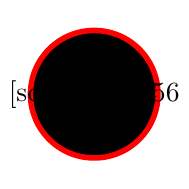
\begin{tikzpicture}[baseline={(current bounding box.center)}]
  \tikzset{pgfornamentstyle/.style={
            draw=Goldenrod,fill=Red,line width=1pt}}
  \node[fill=black,circle,draw=Red,line width=2pt,inner sep=-8pt]
    at (0,0) {\pgfornamenthan[scale=0.38]{56}};
\end{tikzpicture}
\end{tcblisting}

\begin{tcblisting}{title={简单的边框范例}}

\begin{tikzpicture}[x=1pt,y=1pt]
    \tikzset{every node/.append style={inner sep=0pt,color=茜色}}
    \node (nw) {\pgfornamenthan[scale=0.35]{1}};
    \node[anchor=north west,right=140bp of nw] (ne) {\pgfornamenthan[symmetry=v,scale=0.35]{1}};
    \node[anchor=north west,below=0pt of nw] (sw) {\pgfornamenthan[symmetry=h,scale=0.35]{1}};
    \node[anchor=north east,below=0pt of ne] (se) {\pgfornamenthan[symmetry=c,scale=0.35]{1}};

    %% 用 pgfornmanet 自带的 \draw (A) to[ornamenthan=19] (B) 机制的话会导致线条高度跟着变化!只好折衷用tikz的 xscale 来实现加长了。\pgfornamenthan 本身的 scale 则要确保和角点的 scale 一致。
    \node[anchor=south west,xscale=2] at (sw.south east) {\pgfornamenthan[scale=0.35]{29}};

    %% 另外一种方法是用 decorations,同样需要注意一下各种长度参数
    \begin{scope}[decoration={markings,
      mark=between positions 0 and 0.75 step 70bp with
        { \node[transform shape,anchor=north west]{\pgfornamenthan[scale=0.35]{29}};}
      }]
      \draw[decorate] (nw.north east) -- (ne.north west);
    \end{scope}

  \node[font=\kaishu,align=center,xshift=70,text=black] at (nw.south east)
     {给我一片海棠红啊海棠红\\血一样的海棠红\\
     沸血的烧痛是乡愁的烧痛\\给我一片海棠红啊海棠红};
\end{tikzpicture}
\end{tcblisting}

\begin{tcblisting}{title={另一个简单的边框范例}}
\begin{tikzpicture}
  \tikzset{every node/.append style={铜绿,inner sep=0pt}}
  \node (nw) {\pgfornamenthan[scale=0.25]{12}};
  \node[right=50bp of nw] (ne) {\pgfornamenthan[scale=0.25,symmetry=v]{12}};
  \node[below=50bp of nw] (sw) {\pgfornamenthan[scale=0.25,symmetry=h]{12}};
  \node[below=50bp of ne] (se) {\pgfornamenthan[scale=0.25,symmetry=c]{12}};
  % 每个部件原宽度为200bp,因此绘画时如果以bp作为单位,会比较容易计算xscale的值。这里 scale=0.25 则部件有效宽度为50bp,刚好是两个角点符号之间的距离,因此不需要再设 xscale。
  \node[anchor=north west] at (nw.north east) {\pgfornamenthan[scale=0.25]{32}};
  \node[anchor=south west] at (sw.south east) {\pgfornamenthan[scale=0.25]{32}};
  \node[anchor=south west,rotate=-90] at (nw.south west) {\pgfornamenthan[scale=0.25]{32}};
  \node[anchor=south east,rotate=90] at (ne.south east) {\pgfornamenthan[scale=0.25]{32}};

\node[anchor=center,靛蓝,shift={(25bp,-25bp)}] at (nw.south east) {\pgfornamenthan[scale=0.5]{57}};
\end{tikzpicture}
\end{tcblisting}


\begin{tcblisting}{title=有些部件衔接可能需要手动\texttt{shift}}
  \begin{tikzpicture}\tikzset{every node/.append style={赤金,inner sep=0pt}}
    \node (nw) {\pgfornamenthan[scale=0.2]{23}};
    \node[right=53bp of nw] (ne) {\pgfornamenthan[scale=0.2,symmetry=v]{23}};
    \node[anchor=north west,xshift=2bp] at (nw.north east) {\pgfornamenthan[scale=0.2]{41}};
    \node[anchor=north east,xshift=-2bp] at (ne.north west) {\pgfornamenthan[scale=0.2,symmetry=v]{41}};
  \end{tikzpicture}
\end{tcblisting}

\begin{tcblisting}{listing only,title={框着整个页面的代码。很适合拿来设计奖状证书的有木有!}}
  \newbox{\fortyseven}
  \savebox{\fortyseven}{\pgfornamenthan[scale=0.2,color=鸭卵青]{47}}
  \tikzset{every node/.append style={inner sep=0pt,鸭卵青}}
  \begin{tikzpicture}[overlay,remember picture]
  \node[anchor=north west,shift={(14.5pt,-14.5pt)}] at (current page.north west)
    (nw) {\pgfornamenthan[scale=0.2]{25}};
  \node[anchor=north east,shift={(-14.5pt,-14.5pt)}] at (current page.north east)
    (ne) {\pgfornamenthan[scale=0.2,symmetry=v]{25}};
  \node[anchor=south west,shift={(14.5pt,14.5pt)}] at (current page.south west)
    (sw) {\pgfornamenthan[scale=0.2,symmetry=h]{25}};
  \node[anchor=south east,shift={(-14.5pt,14.5pt)}] at (current page.south east)
    (se) {\pgfornamenthan[scale=0.2,symmetry=c]{25}};
  %
  \begin{scope}[start chain,node distance=0pt]
  \node[anchor=north west,on chain] at (nw.north east) {\usebox{\fortyseven}};
  \foreach \i in {1,...,15} {
    \node[on chain]{\usebox{\fortyseven}};
  }
  \end{scope}
  %
  \begin{scope}[start chain,node distance=0pt]
  \node[anchor=south west,on chain] at (sw.south east) {\usebox{\fortyseven}};
  \foreach \i in {1,...,6} \node[on chain]{\usebox{\fortyseven}};
  \end{scope}
  %
  \begin{scope}[start chain=going left,node distance=0pt]
  \node[anchor=south east,on chain] at (se.south west) {\usebox{\fortyseven}};
  \foreach \i in {1,...,6} \node[on chain]{\usebox{\fortyseven}};
  \end{scope}
  %
  % 垂直的话 chains 比较不好控制,我懒得折腾了,直接用 \foreach。
  % 自己算一下, (47) 长度 155. 那么 scale = 0.2 的话……
  \foreach \i in {0,...,21}
    \node[anchor=south west,rotate=-90,shift={($\i*(31bp,0)$)}] at (nw.south west)
      {\usebox{\fortyseven}};
  %
  \foreach \i in {0,...,21}
    \node[anchor=south east,rotate=90,shift={($\i*(-31bp,0)$)}] at (ne.south east)
      {\usebox{\fortyseven}};
  %
  %% 严格来说应该放在 \fancyfoot 吧,算了一样啦
  \node[yshift=32pt,铜绿] at (current page.south) {\pgfornamenthan[scale=0.1]{51}};
  \node[yshift=32pt,text=black] at (current page.south) {\large\thepage};
  %
  \end{tikzpicture}
\end{tcblisting}

\part{纹样列表}

以下部件的原宽度、原高度皆以1bp为单元。


\setlength{\parindent}{0pt}\raggedright

\section{角点符号}

\subsection{接单线的角点符号}

有实心线型与对应的空心线型两种。以下皆同。

\bigskip


\foreach \n in {1,...,8}{%
  \begin{tikzpicture}
    \fill[牙色](-1cm,-1cm) rectangle (1cm,1cm);
    \node[inner sep=0pt] (element) {\pgfornamenthan[color=茜色,width=1.8cm]{\n}};
    \node[inner sep=0pt,font=\footnotesize\bfseries\sffamily,color=紫檀] at (0.8cm,-0.8cm) {\n};
    \node[anchor=west,text width=4em,font=\footnotesize] at (1.1cm,0) {\getpgfornamenthanDim{\n}};
    \draw[color=牙色] (1cm,-1cm) rectangle (2.8cm,1cm);
  \end{tikzpicture}\space\space
}

\subsection{接双线的角点符号}

\foreach \n in {9,...,14}{%
  \begin{tikzpicture}
    \fill[牙色](-1cm,-1cm) rectangle (1cm,1cm);
    \node[inner sep=0pt] (element) {\pgfornamenthan[color=茜色,width=1.8cm]{\n}};
    \node[inner sep=0pt,font=\footnotesize\bfseries\sffamily,color=紫檀] at (0.8cm,-0.8cm) {\n};
    \node[anchor=west,text width=4em,font=\footnotesize] at (1.1cm,0) {\getpgfornamenthanDim{\n}};
    \draw[color=牙色] (1cm,-1cm) rectangle (2.8cm,1cm);
  \end{tikzpicture}\space\space
}


\subsection{简单角点符号}

和其他角点符号配合,在一条对角线上使用其他角点符号,另一条对角 线上使用简单角点符号。

\bigskip

\foreach \n in {15,...,18}{%
  \begin{tikzpicture}
    \fill[牙色](-1cm,-1cm) rectangle (1cm,1cm);
    \node[inner sep=0pt] (element) {\pgfornamenthan[color=茜色,width=1.8cm]{\n}};
    \node[inner sep=0pt,font=\footnotesize\bfseries\sffamily,color=紫檀] at (0.8cm,-0.8cm) {\n};
    \node[anchor=west,text width=4em,font=\footnotesize] at (1.1cm,0) {\getpgfornamenthanDim{\n}};
    \draw[color=牙色] (1cm,-1cm) rectangle (2.8cm,1cm);
  \end{tikzpicture}\space\space
}

\subsection{回纹的角点符号}

和连续的回纹配合。

\bigskip

\foreach \n in {19,...,22}{%
  \begin{tikzpicture}
    \fill[牙色](-1cm,-1cm) rectangle (1cm,1cm);
    \node[inner sep=0pt] (element) {\pgfornamenthan[color=茜色,width=1.8cm]{\n}};
    \node[inner sep=0pt,font=\footnotesize\bfseries\sffamily,color=紫檀] at (0.8cm,-0.8cm) {\n};
    \node[anchor=west,text width=4em,font=\footnotesize] at (1.1cm,0) {\getpgfornamenthanDim{\n}};
    \draw[color=牙色] (1cm,-1cm) rectangle (2.8cm,1cm);
  \end{tikzpicture}\space\space
}

\bigskip\bigskip

和离散的回纹配合。

\bigskip

\foreach \n in {23,...,28}{%
  \begin{tikzpicture}
    \fill[牙色](-1cm,-1cm) rectangle (1cm,1cm);
    \node[inner sep=0pt] (element) {\pgfornamenthan[color=茜色,width=1.8cm]{\n}};
    \node[inner sep=0pt,font=\footnotesize\bfseries\sffamily,color=紫檀] at (0.8cm,-0.8cm) {\n};
    \node[anchor=west,text width=4em,font=\footnotesize] at (1.1cm,0) {\getpgfornamenthanDim{\n}};
    \draw[color=牙色] (1cm,-1cm) rectangle (2.8cm,1cm);
  \end{tikzpicture}\space\space
}


\section{线型单元}

\subsection{单线、双线直线}

\foreach \n in {29,...,32}{%
  \begin{tikzpicture}
    \fill[牙色](-1cm,-1cm) rectangle (1cm,1cm);
    \node[inner sep=0pt] (element) {\pgfornamenthan[color=茜色,width=1.8cm]{\n}};
    \node[inner sep=0pt,font=\footnotesize\bfseries\sffamily,color=紫檀] at (0.8cm,-0.8cm) {\n};
    \node[anchor=west,text width=4em,font=\footnotesize] at (1.1cm,0) {\getpgfornamenthanDim{\n}};
    \draw[color=牙色] (1cm,-1cm) rectangle (2.8cm,1cm);
  \end{tikzpicture}\space\space
}

\subsection{回字纹}

\subsubsection{连续}

\foreach \n in {33,...,36}{%
  \begin{tikzpicture}
    \fill[牙色](-1cm,-1.1cm) rectangle (1cm,0.9cm);
    \node[inner sep=0pt] (element) {\pgfornamenthan[color=茜色,height=0.6cm]{\n}};
    \node[inner sep=0pt,font=\footnotesize\bfseries\sffamily,color=紫檀] at (0.8cm,-0.9cm) {\n};
    \node[anchor=west,text width=4em,font=\footnotesize] at (1.1cm,0) {\getpgfornamenthanDim{\n}};
    \draw[color=牙色] (1cm,-1.1cm) rectangle (2.8cm,0.9cm);
  \end{tikzpicture}\space\space
}%
\foreach \n in {37,...,40}{%
  \begin{tikzpicture}
    \fill[牙色](-1cm,-1.1cm) rectangle (1cm,0.9cm);
    \node[inner sep=0pt] (element) {\pgfornamenthan[color=茜色,height=1.1cm]{\n}};
    \node[inner sep=0pt,font=\footnotesize\bfseries\sffamily,color=紫檀] at (0.8cm,-0.9cm) {\n};
    \node[anchor=west,text width=4em,font=\footnotesize] at (1.1cm,0) {\getpgfornamenthanDim{\n}};
    \draw[color=牙色] (1cm,-1.1cm) rectangle (2.8cm,0.9cm);
  \end{tikzpicture}\space\space
}

\subsubsection{离散}

\foreach \n in {41,...,44}{%
  \begin{tikzpicture}
    \fill[牙色](-1cm,-1.1cm) rectangle (1cm,0.9cm);
    \node[inner sep=0pt] (element) {\pgfornamenthan[color=茜色,height=0.6cm]{\n}};
    \node[inner sep=0pt,font=\footnotesize\bfseries\sffamily,color=紫檀] at (0.8cm,-0.9cm) {\n};
    \node[anchor=west,text width=4em,font=\footnotesize] at (1.1cm,0) {\getpgfornamenthanDim{\n}};
    \draw[color=牙色] (1cm,-1.1cm) rectangle (2.8cm,0.9cm);
  \end{tikzpicture}\space\space
}

\subsubsection{离散连接}

\foreach \n in {45,...,48}{%
  \begin{tikzpicture}
    \fill[牙色](-1cm,-1.1cm) rectangle (1cm,0.9cm);
    \node[inner sep=0pt] (element) {\pgfornamenthan[color=茜色,height=0.6cm]{\n}};
    \node[inner sep=0pt,font=\footnotesize\bfseries\sffamily,color=紫檀] at (0.8cm,-0.9cm) {\n};
    \node[anchor=west,text width=4em,font=\footnotesize] at (1.1cm,0) {\getpgfornamenthanDim{\n}};
    \draw[color=牙色] (1cm,-1.1cm) rectangle (2.8cm,0.9cm);
  \end{tikzpicture}\space\space
}

\subsubsection{圆周排布的回纹}
\foreach \n in {49,...,54}{%
  \begin{tikzpicture}
    \fill[牙色](-1.5cm,-1.5cm) rectangle (1.5cm,1.5cm);
    \node[inner sep=0pt] (element) {\pgfornamenthan[color=茜色,width=2.8cm]{\n}};
    \node[inner sep=0pt,font=\footnotesize\bfseries\sffamily,color=紫檀] at (0,0) {\n};
    \node[anchor=west,text width=4em,font=\footnotesize] at (1.6cm,0) {\getpgfornamenthanDim{\n}};
    \draw[color=牙色] (1.5cm,-1.5cm) rectangle (3.5cm,1.5cm);
  \end{tikzpicture}\space\space
}

\section{吉祥纹路}

\subsection{福字纹}

\foreach \n in {55}{%
  \begin{tikzpicture}
    \fill[牙色](-1cm,-1cm) rectangle (1cm,1cm);
    \node[inner sep=0pt] (element) {\pgfornamenthan[color=茜色,width=1.8cm]{\n}};
    \node[inner sep=0pt,font=\footnotesize\bfseries\sffamily,color=紫檀] at (0.8cm,-0.8cm) {\n};
    \node[anchor=west,text width=4em,font=\footnotesize] at (1.1cm,0) {\getpgfornamenthanDim{\n}};
    \draw[color=牙色] (1cm,-1cm) rectangle (2.8cm,1cm);
  \end{tikzpicture}\space\space
}

\subsection{寿字纹}

\foreach \n in {56,57}{%
  \begin{tikzpicture}
    \fill[牙色](-1cm,-1cm) rectangle (1cm,1cm);
    \node[inner sep=0pt] (element) {\pgfornamenthan[color=茜色,width=1.8cm]{\n}};
    \node[inner sep=0pt,font=\footnotesize\bfseries\sffamily,color=紫檀] at (0.8cm,-0.8cm) {\n};
    \node[anchor=west,text width=4em,font=\footnotesize] at (1.1cm,0) {\getpgfornamenthanDim{\n}};
    \draw[color=牙色] (1cm,-1cm) rectangle (2.8cm,1cm);
  \end{tikzpicture}\space\space
}

\section{云纹}

\subsection{对称符号}

\foreach \n in {58,...,61}{%
\begin{tikzpicture}
  \fill[牙色](-1.5cm,-1cm) rectangle (1.5cm,1cm);
  \node[inner sep=0pt] (element) {\pgfornamenthan[color=茜色,width=2.8cm]{\n}};
  \node[inner sep=0pt,font=\footnotesize\bfseries\sffamily,color=紫檀] at (1.3cm,-0.8cm) {\n};
  \node[anchor=west,text width=4em,font=\footnotesize] at (1.6cm,0) {\getpgfornamenthanDim{\n}};
  \draw[color=牙色] (1.5cm,-1cm) rectangle (3.5cm,1cm);
\end{tikzpicture}\space\space
}


\subsection{左右侧符号}

\foreach \n in {62,...,71}{%
  \begin{tikzpicture}
    \fill[牙色](-1cm,-1cm) rectangle (1cm,1cm);
    \node[inner sep=0pt] (element) {\pgfornamenthan[color=茜色,width=1.8cm]{\n}};
    \node[inner sep=0pt,font=\footnotesize\bfseries\sffamily,color=紫檀] at (0.8cm,-0.8cm) {\n};
    \node[anchor=west,text width=4em,font=\footnotesize] at (1.1cm,0) {\getpgfornamenthanDim{\n}};
    \draw[color=牙色] (1cm,-1cm) rectangle (2.8cm,1cm);
  \end{tikzpicture}\space\space
}


\subsection{角落符号}

\foreach \n in {72,...,75}{%
  \begin{tikzpicture}
    \fill[牙色](-1cm,-1cm) rectangle (1cm,1cm);
    \node[inner sep=0pt] (element) {\pgfornamenthan[color=茜色,width=1.8cm]{\n}};
    \node[inner sep=0pt,font=\footnotesize\bfseries\sffamily,color=紫檀] at (0.8cm,0.8cm) {\n};
    \node[anchor=west,text width=4em,font=\footnotesize] at (1.1cm,0) {\getpgfornamenthanDim{\n}};
    \draw[color=牙色] (1cm,-1cm) rectangle (2.8cm,1cm);
  \end{tikzpicture}\space\space
}

\subsection{连接线}

\foreach \n in {76,...,77}{%
  \begin{tikzpicture}
    \fill[牙色](-1cm,-1cm) rectangle (1cm,1cm);
    \node[inner sep=0pt] (element) {\pgfornamenthan[color=茜色,width=1cm]{\n}};
    \node[inner sep=0pt,font=\footnotesize\bfseries\sffamily,color=紫檀] at (0.8cm,-0.8cm) {\n};
    \node[anchor=west,text width=4em,font=\footnotesize] at (1.1cm,0) {\getpgfornamenthanDim{\n}};
    \draw[color=牙色] (1cm,-1cm) rectangle (2.8cm,1cm);
  \end{tikzpicture}\space\space
}

\section{动物}

\foreach \n in {78,...,78}{%
  \begin{tikzpicture}
    \fill[牙色](-1cm,-1cm) rectangle (1cm,1cm);
    \node[inner sep=0pt] (element) {\pgfornamenthan[color=茜色,width=1.8cm]{\n}};
    \node[inner sep=0pt,font=\footnotesize\bfseries\sffamily,color=紫檀] at (0.8cm,-0.8cm) {\n};
    \node[anchor=west,text width=4em,font=\footnotesize] at (1.1cm,0) {\getpgfornamenthanDim{\n}};
    \draw[color=牙色] (1cm,-1cm) rectangle (2.8cm,1cm);
  \end{tikzpicture}\space\space
}

\vfill

\begin{center}
\begin{tikzpicture}
  \tikzset{every node/.append style={铜绿,inner sep=0pt,node distance=0pt}}
  \node (nw) {\pgfornamenthan[scale=0.2]{6}};
  \node[right=100bp of nw] (ne) {\pgfornamenthan[scale=0.2,symmetry=v]{16}};
  \node[below=-8bp of nw] (sw) {\pgfornamenthan[scale=0.2,symmetry=h]{16}};
  \node[below=-8bp of ne] (se) {\pgfornamenthan[scale=0.2,symmetry=c]{6}};
  \node[anchor=north west,xscale=2.5] at (nw.north east) {\pgfornamenthan[scale=0.2]{30}};
  \node[anchor=south west,xscale=2.5] at (sw.south east) {\pgfornamenthan[scale=0.2]{30}};
  \node[font=\kaishu\Large,text=black,shift={(50bp,4bp)}] at (nw.south east) {待续};
\end{tikzpicture}
\end{center}

\clearpage
\appendix
\setlength{\parindent}{2\ccwd}\justifying
\ctexset{section/name={附录}}
\phantomsection\addcontentsline{toc}{part}{附录}

\section{传统中国颜色 \texttt{cncolours.sty}}

\begingroup


这是我比较早以前做的一个宏包了,最初的色卡取自 \url{http://ylbook.com/cms/web/chuantongsecai/chuantongsecai.htm},只有RGB色值。

 \textbf{(2018年5月)} 感谢网友\href{https://github.com/heangfat}{\emph{端憲}},加入了三正色,以及提供繁体中文的颜色名称。

\medskip

\textbf{(2023年7月)\texttt{cncolours.sty}迎来了2.0更新!}加入了\url{https://www.zhongguose.com}的色卡。这个网站参考的资料是:色谱 中科院科技情报编委会名词室。科学出版社,1957。

载入\texttt{cncolours}宏包时有以下宏包选项:
\begin{itemize}[noitemsep]
  \item 默认(无选项):只定义前面两页(ylbook)的颜色。
  \item \texttt{cas-rgb}:载入zhongguose的RGB颜色值。\emph{若有和ylbook重名的颜色,保留ylbook的颜色值。}
  \item \texttt{cas-rgb*}:同上,\emph{但若有和ylbook重名的颜色,会以zhongguose.com的颜色值覆盖之前的定义。}
  \item \texttt{cas-cmyk}:载入zhongguose的CMYK颜色值。\emph{若有和ylbook重名的颜色,保留ylbook的颜色值。}
  \item \texttt{cas-cmyk*}:同上,\emph{但若有和ylbook重名的颜色,会以zhongguose.com的颜色值覆盖之前的定义。}
\end{itemize}


\bigskip

\renewcommand{\baselinestretch}{2}
\newcommand\showcolour[1]{%
  \fcolorbox{乌黑}{#1}{\makebox[2em]{\phantom{M}}}~\makebox[5em][l]{#1}%
}

\begin{RaggedRight}
\showcolour{粉红}
\showcolour{妃色}
\showcolour{品红}
\showcolour{桃红}
\showcolour{海棠红}
\showcolour{石榴红}
\showcolour{樱桃色}
\showcolour{银红}
\showcolour{大红}
\showcolour{绛紫}
\showcolour{绯红}
\showcolour{胭脂}
\showcolour{朱红}
\showcolour{丹}
\showcolour{彤}
\showcolour{茜色}
\showcolour{火红}
\showcolour{赫赤}
\showcolour{嫣红}
\showcolour{洋红}
\showcolour{炎}
\showcolour{赤}
\showcolour{绾}
\showcolour{枣红}
\showcolour{檀}
\showcolour{殷红}
\showcolour{酡红}
\showcolour{酡颜}
\showcolour{鹅黄}
\showcolour{鸭黄}
\showcolour{樱草色}
\showcolour{杏黄}
\showcolour{杏红}
\showcolour{橘黄}
\showcolour{橙黄}
\showcolour{橘红}
\showcolour{姜黄}
\showcolour{缃色}
\showcolour{橙色}
\showcolour{茶色}
\showcolour{驼色}
\showcolour{昏黄}
\showcolour{栗色}
\showcolour{棕色}
\showcolour{棕绿}
\showcolour{棕黑}
\showcolour{棕红}
\showcolour{棕黄}
\showcolour{赭色}
\showcolour{琥珀}
\showcolour{褐色}
\showcolour{枯黄}
\showcolour{黄栌}
\showcolour{秋色}
\showcolour{秋香色}
\showcolour{嫩绿}
\showcolour{柳黄}
\showcolour{柳绿}
\showcolour{竹青}
\showcolour{葱黄}
\showcolour{葱绿}
\showcolour{葱青}
\showcolour{青葱}
\showcolour{油绿}
\showcolour{绿沉}
\showcolour{碧色}
\showcolour{碧绿}
\showcolour{青碧}
\showcolour{翡翠色}
\showcolour{草绿}
\showcolour{青色}
\showcolour{青翠}
\showcolour{青白}
\showcolour{鸭卵青}
\showcolour{蟹壳青}
\showcolour{鸦青}
\showcolour{绿色}
\showcolour{豆绿}
\showcolour{豆青}
\showcolour{石青}
\showcolour{玉色}
\showcolour{缥}
\showcolour{艾绿}
\showcolour{松柏绿}
\showcolour{松花绿}
\showcolour{松花色}
\showcolour{蓝}
\showcolour{靛青}
\showcolour{靛蓝}
\showcolour{碧蓝}
\showcolour{蔚蓝}
\showcolour{宝蓝}
\showcolour{蓝灰色}
\showcolour{藏青}
\showcolour{藏蓝}
\showcolour{黛}
\showcolour{黛绿}
\showcolour{黛蓝}
\showcolour{黛紫}
\showcolour{紫色}
\showcolour{紫酱}
\showcolour{酱紫}
\showcolour{紫檀}
\showcolour{绀青}
\showcolour{紫棠}
\showcolour{青莲}
\showcolour{群青}
\showcolour{雪青}
\showcolour{丁香色}
\showcolour{藕色}
\showcolour{藕荷色}
\showcolour{苍色}
\showcolour{苍黄}
\showcolour{苍青}
\showcolour{苍黑}
\showcolour{苍白}
\showcolour{水色}
\showcolour{水红}
\showcolour{水绿}
\showcolour{水蓝}
\showcolour{淡青}
\showcolour{湖蓝}
\showcolour{湖绿}
\showcolour{精白}
\showcolour{象牙白}
\showcolour{雪白}
\showcolour{月白}
\showcolour{缟}
\showcolour{素}
\showcolour{荼白}
\showcolour{霜色}
\showcolour{花白}
\showcolour{鱼肚白}
\showcolour{莹白}
\showcolour{灰色}
\showcolour{牙色}
\showcolour{铅白}
\showcolour{玄色}
\showcolour{玄青}
\showcolour{乌色}
\showcolour{乌黑}
\showcolour{漆黑}
\showcolour{墨色}
\showcolour{墨灰}
\showcolour{黑色}
\showcolour{缁色}
\showcolour{煤黑}
\showcolour{黧}
\showcolour{黎}
\showcolour{黝}
\showcolour{黝黑}
\showcolour{黯}
\showcolour{赤金}
\showcolour{金色}
\showcolour{银白}
\showcolour{铜绿}
\showcolour{乌金}
\showcolour{老银}
\showcolour{正青}
\showcolour{正赤}
\showcolour{正黄}
\end{RaggedRight}

\clearpage

\CJKfontspec{Noto Serif CJK TC}
以下是繁體中文字體名稱,由網友\href{https://github.com/heangfat}{\emph{端憲}}提供。姜黃、薑黃是兩種植物。未審此指何種,闕之。

\bigskip

\begin{RaggedRight}
\showcolour{粉紅}
\showcolour{妃色}
\showcolour{品紅}
\showcolour{桃紅}
\showcolour{海棠紅}
\showcolour{石榴紅}
\showcolour{櫻桃色}
\showcolour{銀紅}
\showcolour{大紅}
\showcolour{絳紫}
\showcolour{緋紅}
\showcolour{胭脂}
\showcolour{朱紅}
\showcolour{丹}
\showcolour{彤}
\showcolour{茜色}
\showcolour{火紅}
\showcolour{赫赤}
\showcolour{嫣紅}
\showcolour{洋紅}
\showcolour{炎}
\showcolour{赤}
\showcolour{綰}
\showcolour{棗紅}
\showcolour{檀}
\showcolour{殷紅}
\showcolour{酡紅}
\showcolour{酡顏}
\showcolour{鵝黃}
\showcolour{鴨黃}
\showcolour{櫻草色}
\showcolour{杏黃}
\showcolour{杏紅}
\showcolour{橘黃}
\showcolour{橙黃}
\showcolour{橘紅}
\showcolour{姜黄}
\showcolour{緗色}
\showcolour{橙色}
\showcolour{茶色}
\showcolour{駝色}
\showcolour{昏黃}
\showcolour{栗色}
\showcolour{椶色}
\showcolour{椶綠}
\showcolour{椶黑}
\showcolour{椶紅}
\showcolour{椶黃}
\showcolour{赭色}
\showcolour{琥珀}
\showcolour{褐色}
\showcolour{枯黃}
\showcolour{黃櫨}
\showcolour{秋色}
\showcolour{秋香色}
\showcolour{嫩綠}
\showcolour{柳黃}
\showcolour{柳綠}
\showcolour{竹青}
\showcolour{蔥黃}
\showcolour{蔥綠}
\showcolour{蔥青}
\showcolour{青蔥}
\showcolour{油綠}
\showcolour{綠沉}
\showcolour{碧色}
\showcolour{碧綠}
\showcolour{青碧}
\showcolour{翡翠色}
\showcolour{草綠}
\showcolour{青色}
\showcolour{青翠}
\showcolour{青白}
\showcolour{鴨卵青}
\showcolour{蟹殼青}
\showcolour{鴉青}
\showcolour{綠色}
\showcolour{豆綠}
\showcolour{豆青}
\showcolour{石青}
\showcolour{玉色}
\showcolour{縹}
\showcolour{艾綠}
\showcolour{松柏綠}
\showcolour{松花綠}
\showcolour{松花色}
\showcolour{藍}
\showcolour{靛青}
\showcolour{靛藍}
\showcolour{碧藍}
\showcolour{蔚藍}
\showcolour{寶藍}
\showcolour{藍灰色}
\showcolour{藏青}
\showcolour{藏藍}
\showcolour{黛}
\showcolour{黛綠}
\showcolour{黛藍}
\showcolour{黛紫}
\showcolour{紫色}
\showcolour{紫醬}
\showcolour{醬紫}
\showcolour{紫檀}
\showcolour{紺青}
\showcolour{紫棠}
\showcolour{青蓮}
\showcolour{群青}
\showcolour{雪青}
\showcolour{丁香色}
\showcolour{藕色}
\showcolour{藕荷色}
\showcolour{蒼色}
\showcolour{蒼黃}
\showcolour{蒼青}
\showcolour{蒼黑}
\showcolour{蒼白}
\showcolour{水色}
\showcolour{水紅}
\showcolour{水綠}
\showcolour{水藍}
\showcolour{淡青}
\showcolour{湖藍}
\showcolour{湖綠}
\showcolour{精白}
\showcolour{象牙白}
\showcolour{雪白}
\showcolour{月白}
\showcolour{縞}
\showcolour{素}
\showcolour{荼白}
\showcolour{霜色}
\showcolour{花白}
\showcolour{魚肚白}
\showcolour{瑩白}
\showcolour{灰色}
\showcolour{牙色}
\showcolour{鉛白}
\showcolour{玄色}
\showcolour{玄青}
\showcolour{烏色}
\showcolour{烏黑}
\showcolour{漆黑}
\showcolour{墨色}
\showcolour{墨灰}
\showcolour{黑色}
\showcolour{緇色}
\showcolour{煤黑}
\showcolour{黧}
\showcolour{黎}
\showcolour{黝}
\showcolour{黝黑}
\showcolour{黯}
\showcolour{赤金}
\showcolour{金色}
\showcolour{銀白}
\showcolour{銅綠}
\showcolour{烏金}
\showcolour{老銀}
\showcolour{正青}
\showcolour{正赤}
\showcolour{正黃}
\end{RaggedRight}

\clearpage
\CJKfontspec{Noto Serif CJK SC}
\textbf{\texttt{cas-rgb*} 加载的色值:}
\loadCASrgbcolors*

\begin{RaggedRight}
\showcolour{乳白}
\showcolour{杏仁黄}
\showcolour{茉莉黄}
\showcolour{麦秆黄}
\showcolour{油菜花黄}
\showcolour{佛手黄}
\showcolour{篾黄}
\showcolour{葵扇黄}
\showcolour{柠檬黄}
\showcolour{金瓜黄}
\showcolour{藤黄}
\showcolour{酪黄}
\showcolour{香水玫瑰黄}
\showcolour{淡密黄}
\showcolour{大豆黄}
\showcolour{素馨黄}
\showcolour{向日葵黄}
\showcolour{雅梨黄}
\showcolour{黄连黄}
\showcolour{金盏黄}
\showcolour{蛋壳黄}
\showcolour{肉色}
\showcolour{鹅掌黄}
\showcolour{鸡蛋黄}
\showcolour{鼬黄}
\showcolour{榴萼黄}
\showcolour{淡橘橙}
\showcolour{枇杷黄}
\showcolour{橙皮黄}
\showcolour{北瓜黄}
\showcolour{杏黄}
\showcolour{雄黄}
\showcolour{万寿菊黄}
\showcolour{菊蕾白}
\showcolour{秋葵黄}
\showcolour{硫华黄}
\showcolour{柚黄}
\showcolour{芒果黄}
\showcolour{蒿黄}
\showcolour{姜黄}
\showcolour{香蕉黄}
\showcolour{草黄}
\showcolour{新禾绿}
\showcolour{月灰}
\showcolour{淡灰绿}
\showcolour{草灰绿}
\showcolour{苔绿}
\showcolour{碧螺春绿}
\showcolour{燕羽灰}
\showcolour{蟹壳灰}
\showcolour{潭水绿}
\showcolour{橄榄绿}
\showcolour{蚌肉白}
\showcolour{豆汁黄}
\showcolour{淡茧黄}
\showcolour{乳鸭黄}
\showcolour{荔肉白}
\showcolour{象牙黄}
\showcolour{炒米黄}
\showcolour{鹦鹉冠黄}
\showcolour{木瓜黄}
\showcolour{浅烙黄}
\showcolour{莲子白}
\showcolour{谷黄}
\showcolour{栀子黄}
\showcolour{芥黄}
\showcolour{银鼠灰}
\showcolour{尘灰}
\showcolour{枯绿}
\showcolour{鲛青}
\showcolour{粽叶绿}
\showcolour{灰绿}
\showcolour{鹤灰}
\showcolour{淡松烟}
\showcolour{暗海水绿}
\showcolour{棕榈绿}
\showcolour{米色}
\showcolour{淡肉色}
\showcolour{麦芽糖黄}
\showcolour{琥珀黄}
\showcolour{甘草黄}
\showcolour{初熟杏黄}
\showcolour{浅驼色}
\showcolour{沙石黄}
\showcolour{虎皮黄}
\showcolour{土黄}
\showcolour{百灵鸟灰}
\showcolour{山鸡黄}
\showcolour{龟背黄}
\showcolour{苍黄}
\showcolour{莱阳梨黄}
\showcolour{蜴蜊绿}
\showcolour{松鼠灰}
\showcolour{橄榄灰}
\showcolour{蟹壳绿}
\showcolour{古铜绿}
\showcolour{焦茶绿}
\showcolour{粉白}
\showcolour{落英淡粉}
\showcolour{瓜瓤粉}
\showcolour{蜜黄}
\showcolour{金叶黄}
\showcolour{金莺黄}
\showcolour{鹿角棕}
\showcolour{凋叶棕}
\showcolour{玳瑁黄}
\showcolour{软木黄}
\showcolour{风帆黄}
\showcolour{桂皮淡棕}
\showcolour{猴毛灰}
\showcolour{山鸡褐}
\showcolour{驼色}
\showcolour{茶褐}
\showcolour{古铜褐}
\showcolour{荷花白}
\showcolour{玫瑰粉}
\showcolour{橘橙}
\showcolour{美人焦橙}
\showcolour{润红}
\showcolour{淡桃红}
\showcolour{海螺橙}
\showcolour{桃红}
\showcolour{颊红}
\showcolour{淡罂粟红}
\showcolour{晨曦红}
\showcolour{蟹壳红}
\showcolour{金莲花橙}
\showcolour{草莓红}
\showcolour{龙睛鱼红}
\showcolour{蜻蜓红}
\showcolour{大红}
\showcolour{柿红}
\showcolour{榴花红}
\showcolour{银朱}
\showcolour{朱红}
\showcolour{鲑鱼红}
\showcolour{金黄}
\showcolour{鹿皮褐}
\showcolour{醉瓜肉}
\showcolour{麂棕}
\showcolour{淡银灰}
\showcolour{淡赭}
\showcolour{槟榔综}
\showcolour{银灰}
\showcolour{海鸥灰}
\showcolour{淡咖啡}
\showcolour{岩石棕}
\showcolour{芒果棕}
\showcolour{石板灰}
\showcolour{珠母灰}
\showcolour{丁香棕}
\showcolour{咖啡}
\showcolour{筍皮棕}
\showcolour{燕颔红}
\showcolour{玉粉红}
\showcolour{金驼}
\showcolour{铁棕}
\showcolour{蛛网灰}
\showcolour{淡可可棕}
\showcolour{中红灰}
\showcolour{淡土黄}
\showcolour{淡豆沙}
\showcolour{椰壳棕}
\showcolour{淡铁灰}
\showcolour{中灰驼}
\showcolour{淡栗棕}
\showcolour{可可棕}
\showcolour{柞叶棕}
\showcolour{野蔷薇红}
\showcolour{菠萝红}
\showcolour{藕荷}
\showcolour{陶瓷红}
\showcolour{晓灰}
\showcolour{余烬红}
\showcolour{火砖红}
\showcolour{火泥棕}
\showcolour{绀红}
\showcolour{橡树棕}
\showcolour{海报灰}
\showcolour{玫瑰灰}
\showcolour{火山棕}
\showcolour{豆沙}
\showcolour{淡米粉}
\showcolour{初桃粉红}
\showcolour{介壳淡粉红}
\showcolour{淡藏花红}
\showcolour{瓜瓤红}
\showcolour{芙蓉红}
\showcolour{莓酱红}
\showcolour{法螺红}
\showcolour{落霞红}
\showcolour{淡玫瑰灰}
\showcolour{蟹蝥红}
\showcolour{火岩棕}
\showcolour{赭石}
\showcolour{暗驼棕}
\showcolour{酱棕}
\showcolour{栗棕}
\showcolour{洋水仙红}
\showcolour{谷鞘红}
\showcolour{苹果红}
\showcolour{铁水红}
\showcolour{桂红}
\showcolour{极光红}
\showcolour{粉红}
\showcolour{舌红}
\showcolour{曲红}
\showcolour{红汞红}
\showcolour{淡绯}
\showcolour{无花果红}
\showcolour{榴子红}
\showcolour{胭脂红}
\showcolour{合欢红}
\showcolour{春梅红}
\showcolour{香叶红}
\showcolour{珊瑚红}
\showcolour{萝卜红}
\showcolour{淡茜红}
\showcolour{艳红}
\showcolour{淡菽红}
\showcolour{鱼鳃红}
\showcolour{樱桃红}
\showcolour{淡蕊香红}
\showcolour{石竹红}
\showcolour{草茉莉红}
\showcolour{茶花红}
\showcolour{枸枢红}
\showcolour{秋海棠红}
\showcolour{丽春红}
\showcolour{夕阳红}
\showcolour{鹤顶红}
\showcolour{鹅血石红}
\showcolour{覆盆子红}
\showcolour{貂紫}
\showcolour{暗玉紫}
\showcolour{栗紫}
\showcolour{葡萄酱紫}
\showcolour{牡丹粉红}
\showcolour{山茶红}
\showcolour{海棠红}
\showcolour{玉红}
\showcolour{高粱红}
\showcolour{满江红}
\showcolour{枣红}
\showcolour{葡萄紫}
\showcolour{酱紫}
\showcolour{淡曙红}
\showcolour{唐菖蒲红}
\showcolour{鹅冠红}
\showcolour{莓红}
\showcolour{枫叶红}
\showcolour{苋菜红}
\showcolour{烟红}
\showcolour{暗紫苑红}
\showcolour{殷红}
\showcolour{猪肝紫}
\showcolour{金鱼紫}
\showcolour{草珠红}
\showcolour{淡绛红}
\showcolour{品红}
\showcolour{凤仙花红}
\showcolour{粉团花红}
\showcolour{夹竹桃红}
\showcolour{榲桲红}
\showcolour{姜红}
\showcolour{莲瓣红}
\showcolour{水红}
\showcolour{报春红}
\showcolour{月季红}
\showcolour{豇豆红}
\showcolour{霞光红}
\showcolour{松叶牡丹红}
\showcolour{喜蛋红}
\showcolour{鼠鼻红}
\showcolour{尖晶玉红}
\showcolour{山黎豆红}
\showcolour{锦葵红}
\showcolour{鼠背灰}
\showcolour{甘蔗紫}
\showcolour{石竹紫}
\showcolour{苍蝇灰}
\showcolour{卵石紫}
\showcolour{李紫}
\showcolour{茄皮紫}
\showcolour{吊钟花红}
\showcolour{兔眼红}
\showcolour{紫荆红}
\showcolour{菜头紫}
\showcolour{鹞冠紫}
\showcolour{葡萄酒红}
\showcolour{磨石紫}
\showcolour{檀紫}
\showcolour{火鹅紫}
\showcolour{墨紫}
\showcolour{晶红}
\showcolour{扁豆花红}
\showcolour{白芨红}
\showcolour{嫩菱红}
\showcolour{菠根红}
\showcolour{酢酱草红}
\showcolour{洋葱紫}
\showcolour{海象紫}
\showcolour{绀紫}
\showcolour{古铜紫}
\showcolour{石蕊红}
\showcolour{芍药耕红}
\showcolour{藏花红}
\showcolour{初荷红}
\showcolour{马鞭草紫}
\showcolour{丁香淡紫}
\showcolour{丹紫红}
\showcolour{玫瑰红}
\showcolour{淡牵牛紫}
\showcolour{凤信紫}
\showcolour{萝兰紫}
\showcolour{玫瑰紫}
\showcolour{藤萝紫}
\showcolour{槿紫}
\showcolour{蕈紫}
\showcolour{桔梗紫}
\showcolour{魏紫}
\showcolour{芝兰紫}
\showcolour{菱锰红}
\showcolour{龙须红}
\showcolour{蓟粉红}
\showcolour{电气石红}
\showcolour{樱草紫}
\showcolour{芦穗灰}
\showcolour{隐红灰}
\showcolour{苋菜紫}
\showcolour{芦灰}
\showcolour{暮云灰}
\showcolour{斑鸠灰}
\showcolour{淡藤萝紫}
\showcolour{淡青紫}
\showcolour{青蛤壳紫}
\showcolour{豆蔻紫}
\showcolour{扁豆紫}
\showcolour{芥花紫}
\showcolour{青莲}
\showcolour{芓紫}
\showcolour{葛巾紫}
\showcolour{牵牛紫}
\showcolour{紫灰}
\showcolour{龙睛鱼紫}
\showcolour{荸荠紫}
\showcolour{古鼎灰}
\showcolour{乌梅紫}
\showcolour{深牵牛紫}
\showcolour{银白}
\showcolour{芡食白}
\showcolour{远山紫}
\showcolour{淡蓝紫}
\showcolour{山梗紫}
\showcolour{螺甸紫}
\showcolour{玛瑙灰}
\showcolour{野菊紫}
\showcolour{满天星紫}
\showcolour{锌灰}
\showcolour{野葡萄紫}
\showcolour{剑锋紫}
\showcolour{龙葵紫}
\showcolour{暗龙胆紫}
\showcolour{晶石紫}
\showcolour{暗蓝紫}
\showcolour{景泰蓝}
\showcolour{尼罗蓝}
\showcolour{远天蓝}
\showcolour{星蓝}
\showcolour{羽扇豆蓝}
\showcolour{花青}
\showcolour{睛蓝}
\showcolour{虹蓝}
\showcolour{湖水蓝}
\showcolour{秋波蓝}
\showcolour{涧石蓝}
\showcolour{潮蓝}
\showcolour{群青}
\showcolour{霁青}
\showcolour{碧青}
\showcolour{宝石蓝}
\showcolour{天蓝}
\showcolour{柏林蓝}
\showcolour{海青}
\showcolour{钴蓝}
\showcolour{鸢尾蓝}
\showcolour{牵牛花蓝}
\showcolour{飞燕草蓝}
\showcolour{品蓝}
\showcolour{银鱼白}
\showcolour{安安蓝}
\showcolour{鱼尾灰}
\showcolour{鲸鱼灰}
\showcolour{海参灰}
\showcolour{沙鱼灰}
\showcolour{钢蓝}
\showcolour{云水蓝}
\showcolour{晴山蓝}
\showcolour{靛青}
\showcolour{大理石灰}
\showcolour{海涛蓝}
\showcolour{蝶翅蓝}
\showcolour{海军蓝}
\showcolour{水牛灰}
\showcolour{牛角灰}
\showcolour{燕颔蓝}
\showcolour{云峰白}
\showcolour{井天蓝}
\showcolour{云山蓝}
\showcolour{釉蓝}
\showcolour{鸥蓝}
\showcolour{搪磁蓝}
\showcolour{月影白}
\showcolour{星灰}
\showcolour{淡蓝灰}
\showcolour{鷃蓝}
\showcolour{嫩灰}
\showcolour{战舰灰}
\showcolour{瓦罐灰}
\showcolour{青灰}
\showcolour{鸽蓝}
\showcolour{钢青}
\showcolour{暗蓝}
\showcolour{月白}
\showcolour{海天蓝}
\showcolour{清水蓝}
\showcolour{瀑布蓝}
\showcolour{蔚蓝}
\showcolour{孔雀蓝}
\showcolour{甸子蓝}
\showcolour{石绿}
\showcolour{竹篁绿}
\showcolour{粉绿}
\showcolour{美蝶绿}
\showcolour{毛绿}
\showcolour{蔻梢绿}
\showcolour{麦苗绿}
\showcolour{蛙绿}
\showcolour{铜绿}
\showcolour{竹绿}
\showcolour{蓝绿}
\showcolour{穹灰}
\showcolour{翠蓝}
\showcolour{胆矾蓝}
\showcolour{樫鸟蓝}
\showcolour{闪蓝}
\showcolour{冰山蓝}
\showcolour{虾壳青}
\showcolour{晚波蓝}
\showcolour{蜻蜓蓝}
\showcolour{玉鈫蓝}
\showcolour{垩灰}
\showcolour{夏云灰}
\showcolour{苍蓝}
\showcolour{黄昏灰}
\showcolour{灰蓝}
\showcolour{深灰蓝}
\showcolour{玉簪绿}
\showcolour{青矾绿}
\showcolour{草原远绿}
\showcolour{梧枝绿}
\showcolour{浪花绿}
\showcolour{海王绿}
\showcolour{亚丁绿}
\showcolour{镍灰}
\showcolour{明灰}
\showcolour{淡绿灰}
\showcolour{飞泉绿}
\showcolour{狼烟灰}
\showcolour{绿灰}
\showcolour{苍绿}
\showcolour{深海绿}
\showcolour{长石灰}
\showcolour{苷蓝绿}
\showcolour{莽丛绿}
\showcolour{淡翠绿}
\showcolour{明绿}
\showcolour{田园绿}
\showcolour{翠绿}
\showcolour{淡绿}
\showcolour{葱绿}
\showcolour{孔雀绿}
\showcolour{艾绿}
\showcolour{蟾绿}
\showcolour{宫殿绿}
\showcolour{松霜绿}
\showcolour{蛋白石绿}
\showcolour{薄荷绿}
\showcolour{瓦松绿}
\showcolour{荷叶绿}
\showcolour{田螺绿}
\showcolour{白屈菜绿}
\showcolour{河豚灰}
\showcolour{蒽油绿}
\showcolour{槲寄生绿}
\showcolour{云杉绿}
\showcolour{嫩菊绿}
\showcolour{艾背绿}
\showcolour{嘉陵水绿}
\showcolour{玉髓绿}
\showcolour{鲜绿}
\showcolour{宝石绿}
\showcolour{海沬绿}
\showcolour{姚黄}
\showcolour{橄榄石绿}
\showcolour{水绿}
\showcolour{芦苇绿}
\showcolour{槐花黄绿}
\showcolour{苹果绿}
\showcolour{芽绿}
\showcolour{蝶黄}
\showcolour{橄榄黄绿}
\showcolour{鹦鹉绿}
\showcolour{油绿}
\showcolour{象牙白}
\showcolour{汉白玉}
\showcolour{雪白}
\showcolour{鱼肚白}
\showcolour{珍珠灰}
\showcolour{浅灰}
\showcolour{铅灰}
\showcolour{中灰}
\showcolour{瓦灰}
\showcolour{夜灰}
\showcolour{雁灰}
\showcolour{深灰}
\end{RaggedRight}

\bigskip\bigskip

\textbf{\texttt{cas-cmyk*} 加载的色值:}
\loadCAScmykcolors*

\begin{RaggedRight}
\showcolour{乳白}
\showcolour{杏仁黄}
\showcolour{茉莉黄}
\showcolour{麦秆黄}
\showcolour{油菜花黄}
\showcolour{佛手黄}
\showcolour{篾黄}
\showcolour{葵扇黄}
\showcolour{柠檬黄}
\showcolour{金瓜黄}
\showcolour{藤黄}
\showcolour{酪黄}
\showcolour{香水玫瑰黄}
\showcolour{淡密黄}
\showcolour{大豆黄}
\showcolour{素馨黄}
\showcolour{向日葵黄}
\showcolour{雅梨黄}
\showcolour{黄连黄}
\showcolour{金盏黄}
\showcolour{蛋壳黄}
\showcolour{肉色}
\showcolour{鹅掌黄}
\showcolour{鸡蛋黄}
\showcolour{鼬黄}
\showcolour{榴萼黄}
\showcolour{淡橘橙}
\showcolour{枇杷黄}
\showcolour{橙皮黄}
\showcolour{北瓜黄}
\showcolour{杏黄}
\showcolour{雄黄}
\showcolour{万寿菊黄}
\showcolour{菊蕾白}
\showcolour{秋葵黄}
\showcolour{硫华黄}
\showcolour{柚黄}
\showcolour{芒果黄}
\showcolour{蒿黄}
\showcolour{姜黄}
\showcolour{香蕉黄}
\showcolour{草黄}
\showcolour{新禾绿}
\showcolour{月灰}
\showcolour{淡灰绿}
\showcolour{草灰绿}
\showcolour{苔绿}
\showcolour{碧螺春绿}
\showcolour{燕羽灰}
\showcolour{蟹壳灰}
\showcolour{潭水绿}
\showcolour{橄榄绿}
\showcolour{蚌肉白}
\showcolour{豆汁黄}
\showcolour{淡茧黄}
\showcolour{乳鸭黄}
\showcolour{荔肉白}
\showcolour{象牙黄}
\showcolour{炒米黄}
\showcolour{鹦鹉冠黄}
\showcolour{木瓜黄}
\showcolour{浅烙黄}
\showcolour{莲子白}
\showcolour{谷黄}
\showcolour{栀子黄}
\showcolour{芥黄}
\showcolour{银鼠灰}
\showcolour{尘灰}
\showcolour{枯绿}
\showcolour{鲛青}
\showcolour{粽叶绿}
\showcolour{灰绿}
\showcolour{鹤灰}
\showcolour{淡松烟}
\showcolour{暗海水绿}
\showcolour{棕榈绿}
\showcolour{米色}
\showcolour{淡肉色}
\showcolour{麦芽糖黄}
\showcolour{琥珀黄}
\showcolour{甘草黄}
\showcolour{初熟杏黄}
\showcolour{浅驼色}
\showcolour{沙石黄}
\showcolour{虎皮黄}
\showcolour{土黄}
\showcolour{百灵鸟灰}
\showcolour{山鸡黄}
\showcolour{龟背黄}
\showcolour{苍黄}
\showcolour{莱阳梨黄}
\showcolour{蜴蜊绿}
\showcolour{松鼠灰}
\showcolour{橄榄灰}
\showcolour{蟹壳绿}
\showcolour{古铜绿}
\showcolour{焦茶绿}
\showcolour{粉白}
\showcolour{落英淡粉}
\showcolour{瓜瓤粉}
\showcolour{蜜黄}
\showcolour{金叶黄}
\showcolour{金莺黄}
\showcolour{鹿角棕}
\showcolour{凋叶棕}
\showcolour{玳瑁黄}
\showcolour{软木黄}
\showcolour{风帆黄}
\showcolour{桂皮淡棕}
\showcolour{猴毛灰}
\showcolour{山鸡褐}
\showcolour{驼色}
\showcolour{茶褐}
\showcolour{古铜褐}
\showcolour{荷花白}
\showcolour{玫瑰粉}
\showcolour{橘橙}
\showcolour{美人焦橙}
\showcolour{润红}
\showcolour{淡桃红}
\showcolour{海螺橙}
\showcolour{桃红}
\showcolour{颊红}
\showcolour{淡罂粟红}
\showcolour{晨曦红}
\showcolour{蟹壳红}
\showcolour{金莲花橙}
\showcolour{草莓红}
\showcolour{龙睛鱼红}
\showcolour{蜻蜓红}
\showcolour{大红}
\showcolour{柿红}
\showcolour{榴花红}
\showcolour{银朱}
\showcolour{朱红}
\showcolour{鲑鱼红}
\showcolour{金黄}
\showcolour{鹿皮褐}
\showcolour{醉瓜肉}
\showcolour{麂棕}
\showcolour{淡银灰}
\showcolour{淡赭}
\showcolour{槟榔综}
\showcolour{银灰}
\showcolour{海鸥灰}
\showcolour{淡咖啡}
\showcolour{岩石棕}
\showcolour{芒果棕}
\showcolour{石板灰}
\showcolour{珠母灰}
\showcolour{丁香棕}
\showcolour{咖啡}
\showcolour{筍皮棕}
\showcolour{燕颔红}
\showcolour{玉粉红}
\showcolour{金驼}
\showcolour{铁棕}
\showcolour{蛛网灰}
\showcolour{淡可可棕}
\showcolour{中红灰}
\showcolour{淡土黄}
\showcolour{淡豆沙}
\showcolour{椰壳棕}
\showcolour{淡铁灰}
\showcolour{中灰驼}
\showcolour{淡栗棕}
\showcolour{可可棕}
\showcolour{柞叶棕}
\showcolour{野蔷薇红}
\showcolour{菠萝红}
\showcolour{藕荷}
\showcolour{陶瓷红}
\showcolour{晓灰}
\showcolour{余烬红}
\showcolour{火砖红}
\showcolour{火泥棕}
\showcolour{绀红}
\showcolour{橡树棕}
\showcolour{海报灰}
\showcolour{玫瑰灰}
\showcolour{火山棕}
\showcolour{豆沙}
\showcolour{淡米粉}
\showcolour{初桃粉红}
\showcolour{介壳淡粉红}
\showcolour{淡藏花红}
\showcolour{瓜瓤红}
\showcolour{芙蓉红}
\showcolour{莓酱红}
\showcolour{法螺红}
\showcolour{落霞红}
\showcolour{淡玫瑰灰}
\showcolour{蟹蝥红}
\showcolour{火岩棕}
\showcolour{赭石}
\showcolour{暗驼棕}
\showcolour{酱棕}
\showcolour{栗棕}
\showcolour{洋水仙红}
\showcolour{谷鞘红}
\showcolour{苹果红}
\showcolour{铁水红}
\showcolour{桂红}
\showcolour{极光红}
\showcolour{粉红}
\showcolour{舌红}
\showcolour{曲红}
\showcolour{红汞红}
\showcolour{淡绯}
\showcolour{无花果红}
\showcolour{榴子红}
\showcolour{胭脂红}
\showcolour{合欢红}
\showcolour{春梅红}
\showcolour{香叶红}
\showcolour{珊瑚红}
\showcolour{萝卜红}
\showcolour{淡茜红}
\showcolour{艳红}
\showcolour{淡菽红}
\showcolour{鱼鳃红}
\showcolour{樱桃红}
\showcolour{淡蕊香红}
\showcolour{石竹红}
\showcolour{草茉莉红}
\showcolour{茶花红}
\showcolour{枸枢红}
\showcolour{秋海棠红}
\showcolour{丽春红}
\showcolour{夕阳红}
\showcolour{鹤顶红}
\showcolour{鹅血石红}
\showcolour{覆盆子红}
\showcolour{貂紫}
\showcolour{暗玉紫}
\showcolour{栗紫}
\showcolour{葡萄酱紫}
\showcolour{牡丹粉红}
\showcolour{山茶红}
\showcolour{海棠红}
\showcolour{玉红}
\showcolour{高粱红}
\showcolour{满江红}
\showcolour{枣红}
\showcolour{葡萄紫}
\showcolour{酱紫}
\showcolour{淡曙红}
\showcolour{唐菖蒲红}
\showcolour{鹅冠红}
\showcolour{莓红}
\showcolour{枫叶红}
\showcolour{苋菜红}
\showcolour{烟红}
\showcolour{暗紫苑红}
\showcolour{殷红}
\showcolour{猪肝紫}
\showcolour{金鱼紫}
\showcolour{草珠红}
\showcolour{淡绛红}
\showcolour{品红}
\showcolour{凤仙花红}
\showcolour{粉团花红}
\showcolour{夹竹桃红}
\showcolour{榲桲红}
\showcolour{姜红}
\showcolour{莲瓣红}
\showcolour{水红}
\showcolour{报春红}
\showcolour{月季红}
\showcolour{豇豆红}
\showcolour{霞光红}
\showcolour{松叶牡丹红}
\showcolour{喜蛋红}
\showcolour{鼠鼻红}
\showcolour{尖晶玉红}
\showcolour{山黎豆红}
\showcolour{锦葵红}
\showcolour{鼠背灰}
\showcolour{甘蔗紫}
\showcolour{石竹紫}
\showcolour{苍蝇灰}
\showcolour{卵石紫}
\showcolour{李紫}
\showcolour{茄皮紫}
\showcolour{吊钟花红}
\showcolour{兔眼红}
\showcolour{紫荆红}
\showcolour{菜头紫}
\showcolour{鹞冠紫}
\showcolour{葡萄酒红}
\showcolour{磨石紫}
\showcolour{檀紫}
\showcolour{火鹅紫}
\showcolour{墨紫}
\showcolour{晶红}
\showcolour{扁豆花红}
\showcolour{白芨红}
\showcolour{嫩菱红}
\showcolour{菠根红}
\showcolour{酢酱草红}
\showcolour{洋葱紫}
\showcolour{海象紫}
\showcolour{绀紫}
\showcolour{古铜紫}
\showcolour{石蕊红}
\showcolour{芍药耕红}
\showcolour{藏花红}
\showcolour{初荷红}
\showcolour{马鞭草紫}
\showcolour{丁香淡紫}
\showcolour{丹紫红}
\showcolour{玫瑰红}
\showcolour{淡牵牛紫}
\showcolour{凤信紫}
\showcolour{萝兰紫}
\showcolour{玫瑰紫}
\showcolour{藤萝紫}
\showcolour{槿紫}
\showcolour{蕈紫}
\showcolour{桔梗紫}
\showcolour{魏紫}
\showcolour{芝兰紫}
\showcolour{菱锰红}
\showcolour{龙须红}
\showcolour{蓟粉红}
\showcolour{电气石红}
\showcolour{樱草紫}
\showcolour{芦穗灰}
\showcolour{隐红灰}
\showcolour{苋菜紫}
\showcolour{芦灰}
\showcolour{暮云灰}
\showcolour{斑鸠灰}
\showcolour{淡藤萝紫}
\showcolour{淡青紫}
\showcolour{青蛤壳紫}
\showcolour{豆蔻紫}
\showcolour{扁豆紫}
\showcolour{芥花紫}
\showcolour{青莲}
\showcolour{芓紫}
\showcolour{葛巾紫}
\showcolour{牵牛紫}
\showcolour{紫灰}
\showcolour{龙睛鱼紫}
\showcolour{荸荠紫}
\showcolour{古鼎灰}
\showcolour{乌梅紫}
\showcolour{深牵牛紫}
\showcolour{银白}
\showcolour{芡食白}
\showcolour{远山紫}
\showcolour{淡蓝紫}
\showcolour{山梗紫}
\showcolour{螺甸紫}
\showcolour{玛瑙灰}
\showcolour{野菊紫}
\showcolour{满天星紫}
\showcolour{锌灰}
\showcolour{野葡萄紫}
\showcolour{剑锋紫}
\showcolour{龙葵紫}
\showcolour{暗龙胆紫}
\showcolour{晶石紫}
\showcolour{暗蓝紫}
\showcolour{景泰蓝}
\showcolour{尼罗蓝}
\showcolour{远天蓝}
\showcolour{星蓝}
\showcolour{羽扇豆蓝}
\showcolour{花青}
\showcolour{睛蓝}
\showcolour{虹蓝}
\showcolour{湖水蓝}
\showcolour{秋波蓝}
\showcolour{涧石蓝}
\showcolour{潮蓝}
\showcolour{群青}
\showcolour{霁青}
\showcolour{碧青}
\showcolour{宝石蓝}
\showcolour{天蓝}
\showcolour{柏林蓝}
\showcolour{海青}
\showcolour{钴蓝}
\showcolour{鸢尾蓝}
\showcolour{牵牛花蓝}
\showcolour{飞燕草蓝}
\showcolour{品蓝}
\showcolour{银鱼白}
\showcolour{安安蓝}
\showcolour{鱼尾灰}
\showcolour{鲸鱼灰}
\showcolour{海参灰}
\showcolour{沙鱼灰}
\showcolour{钢蓝}
\showcolour{云水蓝}
\showcolour{晴山蓝}
\showcolour{靛青}
\showcolour{大理石灰}
\showcolour{海涛蓝}
\showcolour{蝶翅蓝}
\showcolour{海军蓝}
\showcolour{水牛灰}
\showcolour{牛角灰}
\showcolour{燕颔蓝}
\showcolour{云峰白}
\showcolour{井天蓝}
\showcolour{云山蓝}
\showcolour{釉蓝}
\showcolour{鸥蓝}
\showcolour{搪磁蓝}
\showcolour{月影白}
\showcolour{星灰}
\showcolour{淡蓝灰}
\showcolour{鷃蓝}
\showcolour{嫩灰}
\showcolour{战舰灰}
\showcolour{瓦罐灰}
\showcolour{青灰}
\showcolour{鸽蓝}
\showcolour{钢青}
\showcolour{暗蓝}
\showcolour{月白}
\showcolour{海天蓝}
\showcolour{清水蓝}
\showcolour{瀑布蓝}
\showcolour{蔚蓝}
\showcolour{孔雀蓝}
\showcolour{甸子蓝}
\showcolour{石绿}
\showcolour{竹篁绿}
\showcolour{粉绿}
\showcolour{美蝶绿}
\showcolour{毛绿}
\showcolour{蔻梢绿}
\showcolour{麦苗绿}
\showcolour{蛙绿}
\showcolour{铜绿}
\showcolour{竹绿}
\showcolour{蓝绿}
\showcolour{穹灰}
\showcolour{翠蓝}
\showcolour{胆矾蓝}
\showcolour{樫鸟蓝}
\showcolour{闪蓝}
\showcolour{冰山蓝}
\showcolour{虾壳青}
\showcolour{晚波蓝}
\showcolour{蜻蜓蓝}
\showcolour{玉鈫蓝}
\showcolour{垩灰}
\showcolour{夏云灰}
\showcolour{苍蓝}
\showcolour{黄昏灰}
\showcolour{灰蓝}
\showcolour{深灰蓝}
\showcolour{玉簪绿}
\showcolour{青矾绿}
\showcolour{草原远绿}
\showcolour{梧枝绿}
\showcolour{浪花绿}
\showcolour{海王绿}
\showcolour{亚丁绿}
\showcolour{镍灰}
\showcolour{明灰}
\showcolour{淡绿灰}
\showcolour{飞泉绿}
\showcolour{狼烟灰}
\showcolour{绿灰}
\showcolour{苍绿}
\showcolour{深海绿}
\showcolour{长石灰}
\showcolour{苷蓝绿}
\showcolour{莽丛绿}
\showcolour{淡翠绿}
\showcolour{明绿}
\showcolour{田园绿}
\showcolour{翠绿}
\showcolour{淡绿}
\showcolour{葱绿}
\showcolour{孔雀绿}
\showcolour{艾绿}
\showcolour{蟾绿}
\showcolour{宫殿绿}
\showcolour{松霜绿}
\showcolour{蛋白石绿}
\showcolour{薄荷绿}
\showcolour{瓦松绿}
\showcolour{荷叶绿}
\showcolour{田螺绿}
\showcolour{白屈菜绿}
\showcolour{河豚灰}
\showcolour{蒽油绿}
\showcolour{槲寄生绿}
\showcolour{云杉绿}
\showcolour{嫩菊绿}
\showcolour{艾背绿}
\showcolour{嘉陵水绿}
\showcolour{玉髓绿}
\showcolour{鲜绿}
\showcolour{宝石绿}
\showcolour{海沬绿}
\showcolour{姚黄}
\showcolour{橄榄石绿}
\showcolour{水绿}
\showcolour{芦苇绿}
\showcolour{槐花黄绿}
\showcolour{苹果绿}
\showcolour{芽绿}
\showcolour{蝶黄}
\showcolour{橄榄黄绿}
\showcolour{鹦鹉绿}
\showcolour{油绿}
\showcolour{象牙白}
\showcolour{汉白玉}
\showcolour{雪白}
\showcolour{鱼肚白}
\showcolour{珍珠灰}
\showcolour{浅灰}
\showcolour{铅灰}
\showcolour{中灰}
\showcolour{瓦灰}
\showcolour{夜灰}
\showcolour{雁灰}
\showcolour{深灰}
\end{RaggedRight}

\endgroup

\clearpage

\section{萧山 Beamer 主题 Xiaoshan Beamer Theme \texttt{beamerthemeXiaoshan.sty}}

这个Beamer主题是以 \href{https://ctan.org/pkg/beamertheme-metropolis}{Metropolis} 为基础,用 \texttt{cncolours.sty} 调了一下颜色,加入少许汉风纹样。

\bigskip

\begin{tcblisting}{listing side comment,title={使用范例},pdf comment={xiaoshan-sample.pdf}}
\documentclass[linespread=1.2,aspectratio=1610]{ctexbeamer}

\usetheme{Xiaoshan}

\author{林莲枝}
\title{萧山Beamer主题}
\subtitle{\texttt{pgfornament-han}附录福利}

\begin{document}

\begin{frame}
  \maketitle
\end{frame}

\section{简介}

\begin{frame}
  \frametitle{其实是 Metropolis 主题的魔改}
  \begin{itemize}
    \item 改了颜色(用了 \texttt{cncolours.sty})
    \item 加入 \texttt{pgfornament-han} 汉风纹样元素
  \end{itemize}
\end{frame}
......
\end{document}
\end{tcblisting}

可以自行查阅\href{https://ctan.org/pkg/beamertheme-metropolis}{Metropolis}的详细宏包手册,有很多可客制化的机制,包括各种元素的配色。

\clearpage

\section{神马浮云 Beamer 主题 Heavenly Clouds Beamer Theme \texttt{beamerthemeHeavenlyClouds.sty}}

这个Beamer主题是我一次病中摸鱼摸出来的,脑洞略大。每一页的背景的云彩纹样,位置、大小、深浅都是随机的,所以如果内容页数比较多,编译时运算可能会比较花时间,请自行斟酌使用此主题。

\bigskip

\begin{tcblisting}{listing side comment,title={使用范例},pdf comment={heavenlyclouds-sample.pdf}}
\documentclass[aspectratio=1610,linespread=1.2]{ctexbeamer}
\usetheme{HeavenlyClouds}

\author{林莲枝}
\title{神马浮云\\Beamer主题}
\subtitle{\texttt{pgfornament-han}附录福利}

\begin{document}

\begin{frame}[noframenumbering]
  \maketitle
\end{frame}

\section{简介一}

\begin{frame}[fragile,allowframebreaks]
  \frametitle{此主题脑洞略大}
  ...
\end{frame}
...
\end{document}
\end{tcblisting}

一些注意事项:
\begin{itemize}
  \item Mac 或 Linux 系统上,\texttt{ctex}是不提供隶书\mintinline{latex}{\lishu}的,请自己设定。例:

  \mintinline{latex}{\providecommand{\lishu}{\CJKfontspec{Libian SC}[BoldFont=Baoli SC,Scale=1.2]}}

  \item 可以用 \mintinline{latex}{\simpleprogressmarker} 以简单圆点代替进度条上的神马。

  \item 标题页的寿字纹,可以用各自高校的标志代替。中国高校校徽很多都是圆形的。确保一下背景是透明色的 png 或 pdf 档就可以了。

  \mintinline{latex}{\titlegraphic{\includegraphics[width=2cm]{logo}}}


  \item 也可以在导言区加一句 \mintinline{latex}{\alttitlecircle},会得到另一种标题页的装饰纹样。效果如下:

  \begin{tikzpicture}%[transform shape,scale=0.5]
    \newbox{\circleelem}%
    \savebox{\circleelem}{%
      \tikzset{pgfornamentstyle/.style={transform shape}}%
      \pgfornamenthan[width=0.5236cm,
         color=殷红!80!black,
         symmetry=h]{74}%
    }
    \begin{scope}[decoration={markings, mark=between positions 0 and 1 step 0.5236cm
    with { \node[transform shape,inner sep=0pt,outer sep=0pt]{\usebox{\circleelem}}; }} ]
    \path [postaction={decorate}] circle (1cm);
    \end{scope}%
    \node {\pgfornamenthan[width=1.25cm,color=殷红]{56}};
  \end{tikzpicture} \emph{效果有可能有点狂,请视场合斟酌使用。}

  \item 一些可以自己更改的颜色:
  \begin{minted}{latex}
  \setbeamercolor{structure}{fg=绀青}
  \setbeamercolor{headline}{fg=群青}
  \setbeamercolor{page number in head/foot}{fg=藏青}
  \setbeamercolor{normal text}{bg=淡青}
  \setbeamercolor{alerted text}{fg=正黄}
  \setbeamercolor{example text}{fg=绿沉}
  \end{minted}
\end{itemize}

\clearpage
\section{天青 Beamer 主题 Tian Qing Beamer Theme \texttt{beamerthemeTianqing.sty}}

几年前看到一个很喜欢的舞台演出,根据个人印象做的一个Beamer主题。本来想取名「青花瓷」的。不过始终没能力重现出来那种感觉啦,眼高手低,惭愧。

(话说拿这个模板去做科研学术性报告,真的不会被导师丢出来吗。)


\bigskip

\begin{tcblisting}{listing side comment,title={使用范例},pdf comment={tianqing-sample.pdf}}
\documentclass[aspectratio=1610,linespread=1.2]{ctexbeamer}
\usetheme{TianQing}

\author{林莲枝}
\title{天青Beamer主题}
\subtitle{\texttt{pgfornament-han}附录福利}

\begin{document}

\begin{frame}
  \maketitle
\end{frame}

\section{基本测试}

\begin{frame}{天青色等烟雨,而我在等你}
    \begin{itemize}
        \item 炊烟袅袅升起, 隔江千万里。...
    \end{itemize}
\end{frame}
...
\end{document}
\end{tcblisting}

如果本地电脑上有比较漂亮的美术字体或书法字体,不妨自己设置一下zhkai,也许会有让人惊喜的效果。例:

\mintinline{latex}|\setCJKfamilyfont{zhkai}{Xingkai SC}|

一些可以自己更改的颜色:
\begin{minted}{latex}
\setbeamercolor{structure}{fg=墨色}
\setbeamercolor{section page}{fg=紫檀}
\setbeamercolor{top deco}{fg=老银}
\setbeamercolor{normal text}{bg=铅白}
\setbeamercolor{alerted text}{fg=玄色}
\setbeamercolor{example text}{fg=鸦青}
\setbeamercolor{block title}{fg=绀青}
\end{minted}

\end{document}
